% =============================================================================
\chapter{Perturbations of Isolated Singularities}
\label{ch:theory}
% =============================================================================
% PURPOSE: the theoretical chapter. It contains no measurements; every example
% in it is computed by hand. It provides (i) the language for the experiments
% (families, local box, convergence notions), (ii) the predictions that
% Chapter 5 tests (rates, singular points, discriminant directions) and (iii)
% the description of the class of surfaces for which a singularity-aware
% method can work (required by the thesis assignment).

Section~\ref{sec:singularities} showed that the regular structure of an
implicit surface breaks down where the gradient vanishes, and
Chapter~\ref{ch:extraction} showed that this is exactly where voxel-based extraction becomes
unreliable. Section~\ref{sec:unfolding} introduced the idea of studying a
degenerate object by embedding it into a family of nearby objects. This
chapter applies that idea to implicit surfaces. We consider one-parameter
families
\[
H_k = F + kG ,
\]
in which the surface $\{F=0\}$ has an isolated singular point and $G$ is a
fixed polynomial, and we ask three questions.
\begin{enumerate}
    \item[(Q1)] In which sense, and how fast, does the surface $\{H_k=0\}$
          approach $\{F=0\}$ as $k\to0$?
    \item[(Q2)] What happens to the singular point? Are new singular points
          created, and if so, how many, where, and of which type?
    \item[(Q3)] Which of these effects can a uniform voxel grid represent?
\end{enumerate}
The chapter is theoretical: results from the literature are quoted with their
source, and only statements derived for this thesis are proved. The numerical
methods that compute the quantities defined here are the subject of
Chapter~\ref{ch:method}, and the measurements are reported in
Chapter~\ref{ch:experiments}.

% -----------------------------------------------------------------------------
\section{One-Parameter Families of Implicit Surfaces}
\label{sec:families}
% PURPOSE: fixes the objects and the notation used in all later chapters,
% including the local box in which everything is measured.

Let $F,G:\mathbb{R}^3\to\mathbb{R}$ be polynomials and put
\begin{equation}
\label{eq:family}
H_k(p)=F(p)+kG(p),\qquad S_k=\{p\in\mathbb{R}^3: H_k(p)=0\},\qquad k\in\mathbb{R}.
\end{equation}
The unperturbed surface is $S_0=\{F=0\}$. We assume that $S_0$ has an
isolated singular point $P$; after a translation, $P$ is the origin. All
statements are local: they concern the part of $S_k$ near the origin, for
small $|k|$. The two one-sided limits $k\to0^-$ and $k\to0^+$ are studied
separately, because they can be different.

\paragraph{The local box.}
Local quantities are measured in the closed box
\begin{equation}
\label{eq:box}
Q_a=\{p\in\mathbb{R}^3:\ \|p\|_\infty\le a\}=[-a,a]^3,\qquad
\|p\|_\infty=\max\{|p_1|,|p_2|,|p_3|\},
\end{equation}
centred at the singular point. A box is used rather than a ball because it is
aligned with the voxel grid of Chapter~\ref{ch:extraction} and with the grid-aligned slices
used for the figures. Nothing in this chapter depends on this choice: since
$\|p\|_\infty\le\|p\|_2\le\sqrt3\,\|p\|_\infty$, every box contains a ball
and is contained in a ball of comparable size, so limits and rates of
convergence are the same for boxes and balls; only constants change.

\begin{definition}[Singular and stationary points]
\label{def:singular-perturbed}
A point $q$ is a \emph{stationary point} of $H_k$ if $\nabla H_k(q)=0$. It is
a \emph{singular point of the surface} $S_k$ if, in addition, $H_k(q)=0$.
\end{definition}

The distinction matters throughout: a perturbation typically creates several
stationary points near the origin, and only those on the zero level are
singular points of the surface (Definition~\ref{def:regular-singular}). A
stationary point with $H_k(q)\neq0$ does not lie on $S_k$.

% -----------------------------------------------------------------------------
\section{Isolated Singularities and Their Local Type}
\label{sec:local-type}
% PURPOSE: before perturbing a singularity we need to know what it is. The
% Milnor number is the single most important invariant here: it bounds the
% number of singular points a perturbation can create (Section 3.6) and it is
% what makes the numerical count of Chapter 4 verifiable.

\subsection{Milnor and Tjurina numbers}

Let $\mathcal{O}$ be the ring of convergent power series in $x,y,z$ (for
polynomials one may equally use the rational functions whose denominator does
not vanish at the origin), and let $F\in\mathcal{O}$ with $F(0)=0$.

\begin{definition}[Milnor and Tjurina numbers \cite{milnor1968singular,greuel2007introduction}]
\label{def:milnor}
The \emph{Milnor algebra} and the \emph{Tjurina algebra} of $F$ at the origin are
\[
M_F=\mathcal{O}\big/\big(\partial_xF,\partial_yF,\partial_zF\big),\qquad
T_F=\mathcal{O}\big/\big(F,\partial_xF,\partial_yF,\partial_zF\big),
\]
and their dimensions as real vector spaces are the \emph{Milnor number}
$\mu(F)$ and the \emph{Tjurina number} $\tau(F)$.
\end{definition}

The origin is an isolated singular point of $F$ (more precisely, an isolated
zero of $\nabla F$) exactly when $\mu(F)<\infty$ \cite{greuel2007introduction}.
Always $\tau\le\mu$, with equality if and only if $F$ is
\emph{quasi-homogeneous} in suitable local coordinates
\cite{saito1971quasihomogene}: there are weights $w_1,w_2,w_3>0$ with
\begin{equation}
\label{eq:quasihomogeneous}
F(t^{w_1}x,t^{w_2}y,t^{w_3}z)=t\,F(x,y,z)\qquad\text{for all }t>0.
\end{equation}
A homogeneous polynomial of degree $d$ is quasi-homogeneous with all weights
equal to $1/d$. For the cubic $F_+=x^3+y^3+z^3$ the ideal
$(\partial_xF,\partial_yF,\partial_zF)=(x^2,y^2,z^2)$ is generated by monomials,
and the monomials not divisible by $x^2$, $y^2$ or $z^2$,
\begin{equation}
\label{eq:milnor-basis}
1,\ x,\ y,\ z,\ xy,\ xz,\ yz,\ xyz,
\end{equation}
form a basis of $M_F$; hence $\mu(F_+)=8$. Since $3F=x\partial_xF+y\partial_yF+z\partial_zF$
(Euler's identity), $F$ lies in its own gradient ideal and $\tau(F_+)=\mu(F_+)=8$.

\subsection{Normal forms}

Two germs are \emph{right equivalent} if one becomes the other after a local
change of coordinates. Isolated singularities of small Milnor number are
classified up to right equivalence by normal forms
\cite{arnold2012singularities}; Table~\ref{tab:normal-forms} lists the types
needed here. The simple elliptic singularity $\tilde E_6$ is the cone over a
smooth plane cubic curve; it comes in a one-parameter family, since the
modulus of the elliptic curve cannot be changed by coordinate changes.
Among the singular points of cubic surfaces, $\tilde E_6$ is the most
degenerate isolated one; the others are $A_1,\dots,A_5$, $D_4$, $D_5$ and
$E_6$ \cite{bruce1979classification}.

\begin{table}[!h]
\centering
\small
\begin{tabular}{l l c l}
\toprule
Type & Normal form & $\mu$ & Weights $(w_x,w_y,w_z)$ \\
\midrule
$A_1$ & $x^2+y^2+z^2$ (signs may vary) & $1$ & $(\frac12,\frac12,\frac12)$ \\
$A_2$ & $x^2+y^2+z^3$ & $2$ & $(\frac12,\frac12,\frac13)$ \\
$D_4$ & $x^2+y^3+z^3$, \ $x^2+y^3-3yz^2$ & $4$ & $(\frac12,\frac13,\frac13)$ \\
$\tilde E_6$ & $x^3+y^3+z^3+t\,xyz$, \ $t^3\neq-27$ & $8$ & $(\frac13,\frac13,\frac13)$ \\
\bottomrule
\end{tabular}
\caption[Normal forms]{Normal forms of the singularity types used in this
thesis \cite{arnold2012singularities}. Over the real numbers $A_1$ and $D_4$
have several forms that differ by signs; the two $D_4$ forms differ in the
number of real linear factors of their cubic part: one for $y^3+z^3$, three
for $y^3-3yz^2$.}
\label{tab:normal-forms}
\end{table}

\subsection{The reference surfaces}
\label{sec:reference-surfaces}

The experiments of Chapter~\ref{ch:experiments} use the ten surfaces of
Table~\ref{tab:reference-surfaces}, which cover all four types. Their types
can be read off by hand.
\begin{itemize}
    \item $x^2+y^2-z^2+xyz$ has a nondegenerate Hessian at the origin, so by the
          Morse lemma \cite{milnor1963morse} it is an ordinary double point
          $A_1$; the cubic term does not change the type.
    \item $x^2\pm y^2+z^3$ are normal forms of $A_2$. In
          $x^3+y^3+z^2+x^2=x^2(1+x)+z^2+y^3$ the factor $1+x$ is positive near
          the origin, and the substitution $\tilde x=x\sqrt{1+x}$ gives the
          normal form $\tilde x^2+z^2+y^3$: again $A_2$, now with the cubic
          direction along $y$.
    \item $x^2+y^3+z^3$ and $x^2+y^3-3yz^2$ are the two real normal forms of
          $D_4$: the cubic part $y^3+z^3$ has one real linear factor,
          $y^3-3yz^2=y(y-\sqrt3z)(y+\sqrt3z)$ has three.
    \item The four homogeneous cubics are cones over plane cubic curves. Such a
          cone has an isolated singular point exactly when the curve is smooth
          \cite{dimca1992singularities}. The Fermat curves $x^3+y^3\pm z^3=0$
          and the Hesse curve $x^3+y^3+z^3+t\,xyz=0$ with $t=1$ (smooth for
          $t^3\neq-27$) are smooth; for $x^3+2y^3+3z^3+2xyz$ the computation of
          Section~\ref{sec:method-algebra} gives $\mu=8$, so it is of type
          $\tilde E_6$ as well.
\end{itemize}

\begin{table}[!h]
\centering
\small
\begin{tabular}{l l c c l}
\toprule
Type & $F$ & $\mu$ & $\tau$ & Monomial basis of $T_F$ \\
\midrule
$A_1$ & $x^2+y^2-z^2+xyz$ & 1 & 1 & $1$ \\
$A_2$ & $x^2+y^2+z^3$ & 2 & 2 & $1,\ z$ \\
$A_2$ & $x^2-y^2+z^3$ & 2 & 2 & $1,\ z$ \\
$A_2$ & $x^3+y^3+z^2+x^2$ & 2 & 2 & $1,\ y$ \\
$D_4$ & $x^2+y^3+z^3$ & 4 & 4 & $1,\ y,\ z,\ yz$ \\
$D_4$ & $x^2+y^3-3yz^2$ & 4 & 4 & $1,\ y,\ z,\ z^2$ \\
$\tilde E_6$ & $F_+=x^3+y^3+z^3$ & 8 & 8 & $1,x,y,z,xy,xz,yz,xyz$ \\
$\tilde E_6$ & $F_-=x^3+y^3-z^3$ & 8 & 8 & $1,x,y,z,xy,xz,yz,xyz$ \\
$\tilde E_6$ & $x^3+y^3+z^3+xyz$ & 8 & 8 & $1,x,y,z,y^2,yz,z^2,z^3$ \\
$\tilde E_6$ & $x^3+2y^3+3z^3+2xyz$ & 8 & 8 & $1,x,y,z,y^2,yz,z^2,z^3$ \\
\bottomrule
\end{tabular}
\caption[Reference surfaces]{The ten reference surfaces, all with an isolated
singular point at the origin. The Milnor and Tjurina numbers and the bases were
computed with the method of Section~\ref{sec:method-algebra} and agree with the
types derived above. A basis is not unique; the method chooses monomials of
the lowest possible degree.}
\label{tab:reference-surfaces}
\end{table}

\subsection{Why the cubic surfaces are called cones}
\label{sec:cones}

A homogeneous polynomial of degree $d$ satisfies $F(tp)=t^dF(p)$ for every
real $t$. Hence if $p$ lies on $S_0$, so does every point $tp$: $S_0$ is a
union of straight lines through the origin. This is the algebraic meaning of
the word \emph{cone} \cite{dimca1992singularities}: the cone over the curve
$C=S_0\cap\{\|p\|_2=1\}$, or equivalently over the projective plane curve
$\{F=0\}\subset\mathbb{RP}^2$. It does not mean that the surface looks like
the familiar circular cone. The shape depends on the curve.
\begin{itemize}
    \item Over a circle, for example $x^2+y^2=z^2$, one obtains the familiar
          double cone (Figure~\ref{fig:cone} in Chapter~1).
    \item Over a projective line, for example $x=0$, one obtains a plane.
    \item The real Fermat cubic $x^3+y^3+z^3=0$ is a single curve in
          $\mathbb{RP}^2$: in the chart $z=1$ it is the graph
          $y=-\sqrt[3]{1+x^3}$ of a continuous function, closed up by the one
          point $(1:-1:0)$ at infinity. Like a projective line, it cannot be
          contracted to a point. The cone over it is therefore a single
          connected sheet through the origin that resembles a twisted plane.
          It is smooth everywhere except at the origin, where all its lines
          meet (Figure~\ref{fig:reference-cones}).
\end{itemize}
Non-homogeneous surfaces such as $x^2+y^2-z^2+xyz$ are not cones, but near
the singular point they are approximated by one: the zero set of the
lowest-order homogeneous part of $F$, the \emph{tangent cone}
\cite{dimca1992singularities}. For the surfaces of type $A_2$ and $D_4$ the
tangent cone is degenerate (a line or a doubled plane), and the weighted
homogeneity \eqref{eq:quasihomogeneous} takes over its role.

\begin{figure}[!h]
    \centering
    \begin{subfigure}{0.47\textwidth}
        \centering
        \thesisimage{pictures/ch3/cone_Fplus.png}{\textwidth}{5cm}{$S_0$ for $F_+=x^3+y^3+z^3$, 3D view coloured by $\|\nabla F\|$}
        \caption{$F_+=x^3+y^3+z^3$}
    \end{subfigure}
    \hfill
    \begin{subfigure}{0.47\textwidth}
        \centering
        \thesisimage{pictures/ch3/cone_Fminus.png}{\textwidth}{5cm}{$S_0$ for $F_-=x^3+y^3-z^3$, same view and colour scale}
        \caption{$F_-=x^3+y^3-z^3$}
    \end{subfigure}
    \caption[Cubic cones]{Two cubic cones. Each is a single sheet made of
    lines through the origin; the colour encodes $\|\nabla F\|$, which
    vanishes only at the apex.}
    \label{fig:reference-cones}
\end{figure}

The two Fermat cones are related by the reflection $\rho(x,y,z)=(x,y,-z)$:
$F_-=F_+\circ\rho$, hence
\begin{equation}
\label{eq:reflection}
F_-+kG=\big(F_++k\,(G\circ\rho)\big)\circ\rho .
\end{equation}
A result for $F_+$ and the perturbation $G\circ\rho$ is therefore a result for
$F_-$ and $G$, mirrored. A fixed perturbation such as $x+z$, however, is a
different perturbation for the two cones.

% -----------------------------------------------------------------------------
\section{The Singular Point Under Perturbation}
\label{sec:point-under-perturbation}
% PURPOSE: the first, purely local answer to (Q2): what happens AT the
% singular point. Only the value, gradient and Hessian of G at P are needed;
% this is the only place where Taylor expansions are used.

At the origin $F$ and $\nabla F$ vanish, so
\begin{equation}
\label{eq:at-origin}
H_k(0)=kG(0),\qquad \nabla H_k(0)=k\nabla G(0),\qquad
\operatorname{Hess}H_k(0)=\operatorname{Hess}F(0)+k\operatorname{Hess}G(0).
\end{equation}
For every $k\neq0$ this decides the fate of the origin:
\begin{itemize}
    \item if $G(0)\neq0$, the origin \emph{leaves} the surface;
    \item if $G(0)=0$ and $\nabla G(0)\neq0$, it stays on $S_k$ as a
          \emph{regular} point, with gradient of size $|k|\,\|\nabla G(0)\|$;
    \item if $G(0)=0$ and $\nabla G(0)=0$, it \emph{stays singular}; its type
          is decided by the Hessian and higher terms. For example
          $F_++kx^2$ has the leading terms $kx^2+y^3+z^3$, which is the
          normal form of $D_4$: the singular point persists but becomes
          simpler ($\mu=4$ instead of $8$).
\end{itemize}
None of these tests excludes singular points away from the origin; those are
the subject of Sections~\ref{sec:vector} and~\ref{sec:linear}.

\begin{definition}[Order of a perturbation]
\label{def:order}
Write $G=G_0+G_1+G_2+\cdots$, with $G_j$ homogeneous of degree $j$. The
\emph{order} of $G$ is the smallest $m$ with $G_m\neq0$. If $F$ is
quasi-homogeneous with weights $w$, the \emph{weighted order} $d_w(G)$ is the
smallest value of $w_1i+w_2j+w_3l$ over the monomials $x^iy^jz^l$ of $G$.
\end{definition}

The order is local and need not equal the degree: $G=x^2+x$ has degree two
but order one. Of the Taylor expansion of $G$ only the terms up to order two
are needed in this thesis: the value, the gradient and the Hessian at the
singular point. They decide the three cases above and, through the order, the
scale of the deformation (next section).

% -----------------------------------------------------------------------------
\section{Notions of Convergence}
\label{sec:convergence-notions}
% PURPOSE: "S_k converges to S_0" has several precise meanings, and the
% experiments measure several of them. This section defines them and states
% what is guaranteed without any computation.

\begin{definition}[Local Hausdorff distance]
\label{def:local-hausdorff}
For closed sets $A,B\subset\mathbb{R}^3$ and the box $Q_a$ of~\eqref{eq:box},
\[
d_a(A,B)=\max\Big\{\sup_{p\in A\cap Q_a}\operatorname{dist}(p,B),\
\sup_{p\in B\cap Q_a}\operatorname{dist}(p,A)\Big\},\qquad
\operatorname{dist}(p,B)=\inf_{q\in B}\|p-q\|_2 ,
\]
with the convention $\sup\emptyset=0$. We write $d_a(k)=d_a(S_k,S_0)$.
\end{definition}

The points are taken in the box, but their distance is measured to the whole
other set. Distances to the parts of the other set just outside the box are
therefore not counted as errors. For $a=\infty$ this is the usual Hausdorff
distance \cite{rockafellar1998variational}.

\begin{definition}[Notions of convergence]
\label{def:convergence-types}
Let $k\to0$ from one side.
\begin{enumerate}
    \item \textbf{Set convergence.} $S_k\to S_0$ in $Q_a$ if every point of
          $S_0\cap Q_a$ is a limit of points of $S_k$, and every limit of
          points of $S_k\cap Q_a$ lies in $S_0$ (Painlevé--Kuratowski
          convergence \cite{rockafellar1998variational}).
    \item \textbf{Convergence with rate $\alpha$.} $d_a(k)=\Theta(|k|^\alpha)$,
          that is, $c|k|^\alpha\le d_a(k)\le C|k|^\alpha$ for small $|k|$. The
          convergence is \emph{Lipschitz} if $\alpha=1$ and \emph{Hölder} if
          $0<\alpha<1$.
    \item \textbf{Convergence of singular points.} Singular points $q(k)$ of
          $S_k$ converge to the origin with rate $\gamma$ if
          $\|q(k)\|=\Theta(|k|^\gamma)$.
\end{enumerate}
\end{definition}

These notions can disagree. If $G(0)=0$, the origin stays on $S_k$, so the
distance from the origin to $S_k$ is zero for every $k$, although the surface
changes. New singular points can converge to the origin while the origin
itself becomes regular. Two facts hold without computation. First, every
limit of points $q_k\in S_k\cap Q_a$ lies on $S_0$, for every $G$: since $G$
is bounded on $Q_a$, $F(q_k)=-kG(q_k)\to0$. Second, if $F$ takes both signs
in every neighbourhood of a point $p\in S_0$, then $S_k$ meets every
neighbourhood of $p$ for small $|k|$: pick $a,b$ near $p$ with
$F(a)<0<F(b)$; for $|k|$ small enough $H_k$ keeps these signs, and by the
intermediate value theorem it vanishes on the segment $[a,b]$. For an odd
polynomial, $F(-p)=-F(p)$, such as the Fermat cones, the second condition holds
at every point of $S_0$. Hence:

\begin{proposition}
\label{prop:set-convergence}
For the cubic cones $F_\pm$, $S_k$ converges to $S_0$ in the sense of sets from
both sides of $k=0$, for every polynomial $G$.
\end{proposition}

Set convergence fails only where $F$ does not change sign. For
$x^2+y^2+z^2+k$ the surface is empty for $k>0$ and a sphere of radius
$\sqrt{|k|}$ for $k<0$, so the convergence is one-sided.

A universal bound on the rate follows from the \emph{Łojasiewicz inequality}
\cite{lojasiewicz1959division,bochnak1998real}: for a polynomial $F$ and a
compact set $K$ there are $c>0$ and an exponent $\ell\ge1$ with
$|F(p)|\ge c\operatorname{dist}(p,S_0)^\ell$ on $K$. On $S_k$ we have
$|F|=|k||G|$, so no point of $S_k\cap K$ is farther than
$(|k|\max_K|G|/c)^{1/\ell}$ from $S_0$. For a homogeneous cubic with
$\nabla F\neq0$ away from the origin one can take $\ell=3$ (by homogeneity,
it suffices to check the inequality on the unit sphere), so one half of the
local Hausdorff distance is always $O(|k|^{1/3})$. The precise rate is given
by a scaling argument.

% -----------------------------------------------------------------------------
\section{Scaling and the Model Surface}
\label{sec:scaling}
% PURPOSE: the core prediction of the thesis. It explains WHY the rates are
% 1/3, 1/2, 1 and where the deformation happens (the inner region), and it
% links Chapter 1's blowup to implicit surfaces. Section 3.5.1 builds the
% idea in one variable, 3.5.2 in three, 3.5.3 proves the exact case, 3.5.4
% states the general case as a principle that Chapter 5 tests.

\subsection{The idea in one variable}

Consider $f_k(x)=x^3+kx$. For $k=0$ its only zero is $x=0$, a triple zero.
For $k<0$ there are three zeros, $0$ and $\pm\sqrt{-k}$; for $k>0$ only $0$
remains, but the graph turns from a horizontal inflection into a steep
crossing (Figure~\ref{fig:one-variable}). Both changes happen at the same
length scale $|x|\approx\sqrt{|k|}$, which can be predicted without solving
anything: the two terms $x^3$ and $kx$ are of equal size when
$|x|^3=|k|\,|x|$, that is, $|x|=|k|^{1/2}$. For $|x|\gg|k|^{1/2}$ the cubic
term dominates and $f_k$ looks like $f_0$; for $|x|\ll|k|^{1/2}$ the
perturbation dominates. The same balance for $f_k(x)=x^3+k$ gives
$|x|^3=|k|$, the scale $|k|^{1/3}$, and indeed the zero is $x=-k^{1/3}$.

\begin{figure}[!h]
\centering
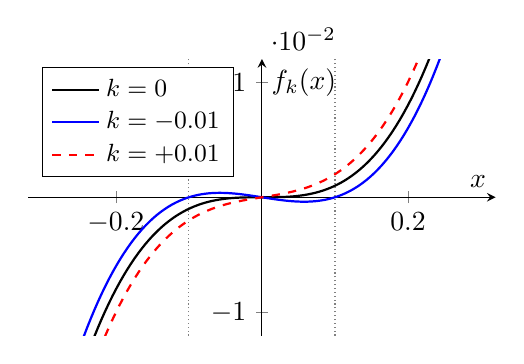
\begin{tikzpicture}
\begin{axis}[width=0.62\textwidth, height=0.42\textwidth,
    xlabel={$x$}, ylabel={$f_k(x)$}, xmin=-0.32, xmax=0.32, ymin=-0.012, ymax=0.012,
    axis lines=middle, legend pos=north west, legend cell align=left,
    legend style={font=\small}, yticklabel style={/pgf/number format/fixed}]
\addplot[black, thick, domain=-0.3:0.3, samples=120] {x^3};
\addlegendentry{$k=0$}
\addplot[blue, thick, domain=-0.3:0.3, samples=120] {x^3-0.01*x};
\addlegendentry{$k=-0.01$}
\addplot[red, thick, dashed, domain=-0.3:0.3, samples=120] {x^3+0.01*x};
\addlegendentry{$k=+0.01$}
\addplot[gray, densely dotted] coordinates {(-0.1,-0.012) (-0.1,0.012)};
\addplot[gray, densely dotted] coordinates {(0.1,-0.012) (0.1,0.012)};
\end{axis}
\end{tikzpicture}
\caption[Scaling in one variable]{$f_k(x)=x^3+kx$. The changes caused by the
perturbation are confined to $|x|\lesssim\sqrt{|k|}=0.1$ (dotted lines);
outside, the three graphs are almost the same.}
\label{fig:one-variable}
\end{figure}

\subsection{Rescaling in three variables}

Let $F$ be homogeneous of degree $d$ with $\nabla F\neq0$ away from the
origin (for the cubic cones $d=3$), and let $G$ have order $m<d$. The balance
$|p|^d=|k|\,|p|^m$ gives the \emph{characteristic scale}
\begin{equation}
\label{eq:scale}
\lambda(k)=|k|^{1/(d-m)} .
\end{equation}
Substituting $p=\lambda u$ and dividing by $\lambda^d$, with $\sigma=\operatorname{sign}k$,
\begin{equation}
\label{eq:rescaled}
\frac{H_k(\lambda u)}{\lambda^d}=F(u)+\sigma\,G_m(u)+O(\lambda),
\end{equation}
because $kG_m(\lambda u)/\lambda^d=\sigma\lambda^{m-d}|k|\,G_m(u)=\sigma G_m(u)$,
and the higher terms $G_{m+1},G_{m+2},\dots$ carry extra factors of $\lambda$.
In the coordinates $u=p/\lambda$ the surfaces therefore approach the fixed
\emph{model surface}
\begin{equation}
\label{eq:model}
M_\sigma=\{u\in\mathbb{R}^3:\ F(u)+\sigma G_m(u)=0\}.
\end{equation}
Geometrically, $S_k$ near the origin is a copy of $M_\sigma$ shrunk by the
factor $\lambda(k)$ (the \emph{inner region}, $\|p\|\lesssim\lambda$), while
farther away it is a small displacement of the cone $S_0$ (the \emph{outer
region}); see Figure~\ref{fig:inner-outer}. Singular points of $S_k$ near the
origin correspond to singular points of $M_\sigma$: if $M_\sigma$ is smooth,
$S_k$ is smooth near the origin, and a singular point $u^\ast$ of $M_\sigma$
appears in $S_k$ at $\lambda u^\ast$, converging to the origin with rate
$\gamma=1/(d-m)$.

\begin{figure}[!h]
\centering
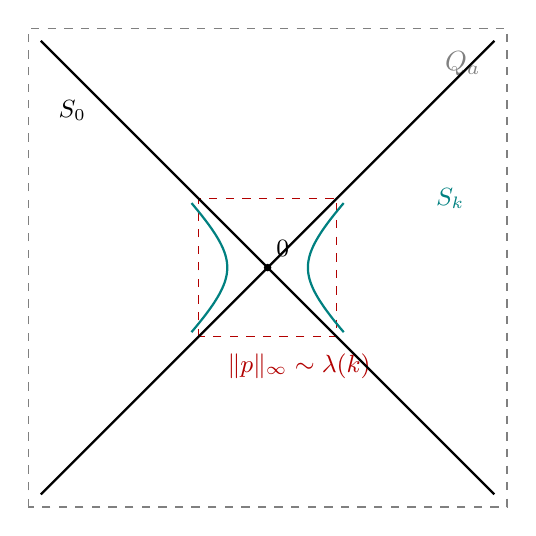
\begin{tikzpicture}[scale=1.6]
    \draw[dashed, gray] (-1.9,-1.9) rectangle (1.9,1.9);
    \node[gray] at (1.55,1.62) {$Q_a$};
    \draw[dashed, red!70!black] (-0.55,-0.55) rectangle (0.55,0.55);
    \node[red!70!black, font=\small] at (0.25,-0.78) {$\|p\|_\infty\sim\lambda(k)$};
    \draw[thick, black] (-1.8,-1.8) -- (1.8,1.8);
    \draw[thick, black] (-1.8,1.8) -- (1.8,-1.8);
    \node[font=\small] at (-1.55,1.25) {$S_0$};
    \draw[thick, teal, domain=-1.25:1.25, samples=60, smooth] plot ({0.32*cosh(\x)}, {0.32*sinh(\x)});
    \draw[thick, teal, domain=-1.25:1.25, samples=60, smooth] plot ({-0.32*cosh(\x)}, {0.32*sinh(\x)});
    \node[teal, font=\small] at (1.45,0.55) {$S_k$};
    \fill (0,0) circle (0.03);
    \node[font=\small] at (0.12,0.15) {$0$};
\end{tikzpicture}
\caption[Inner and outer region]{Schematic cross-section. In the inner region,
of size proportional to $\lambda(k)$, $S_k$ is a scaled copy of the model
surface $M_\sigma$, which here has opened the singular point. In the outer
region $S_k$ stays close to the cone $S_0$.}
\label{fig:inner-outer}
\end{figure}

\subsection{The exact case: homogeneous perturbations}

When $G$ is itself homogeneous, the error term in~\eqref{eq:rescaled}
vanishes and the description becomes exact.

\begin{proposition}[Self-similarity]
\label{prop:self-similar}
Let $F$ be homogeneous of degree $d$ and $G$ homogeneous of degree $m<d$, let
$k\neq0$, $\sigma=\operatorname{sign}k$ and $\lambda=|k|^{1/(d-m)}$. Then
\begin{enumerate}
    \item $S_k=\lambda M_\sigma$, where $M_\sigma=\{F+\sigma G=0\}$;
    \item $d_a(S_k,S_0)=\lambda\,d_{a/\lambda}(M_\sigma,S_0)$, and
          $d_a(S_k,S_0)/\lambda$ increases to the Hausdorff distance
          $C_\sigma=d_\infty(M_\sigma,S_0)$ as $k\to0^\sigma$.
\end{enumerate}
Consequently, if $0<C_\sigma<\infty$, then $d_a(k)=C_\sigma|k|^{1/(d-m)}(1+o(1))$:
the rate of convergence is exactly $\alpha=1/(d-m)$.
\end{proposition}

\begin{proof}
(1) $H_k(\lambda u)=\lambda^dF(u)+k\lambda^mG(u)=\lambda^d\big(F(u)+\sigma G(u)\big)$.
(2) The cone satisfies $S_0=\lambda S_0$, and $\lambda Q_{a/\lambda}=Q_a$, so
all points and distances in Definition~\ref{def:local-hausdorff} scale by
$\lambda$. The box $Q_{a/\lambda}$ grows as $\lambda\to0$, and $d_b$ is
nondecreasing in $b$, with limit $d_\infty$.
\end{proof}

For the constant perturbation $G=1$ ($m=0$) and the cubic cones, the model
surface $\{F=-\sigma\}$ approaches the cone at infinity, so $C_\sigma$ is
finite, and the rate is exactly $1/3$. For a linear $G$ the rate is exactly
$1/2$, and for a homogeneous quadratic $G$ exactly $1$. The constant
$C_\sigma$ depends on the direction of $G$, not only on its order; it is
measured in Chapter~\ref{ch:experiments}. The proposition also predicts a
picture: the zero sets for $k$, $4k$ and $16k$ ($d-m=2$) are identical up to
the factor $2$ in each step, which Section~\ref{sec:exp-self-similarity} uses
as a visual test.

\subsection{The general case}

For a non-homogeneous $G$, such as $x^2+x$, the higher terms in
\eqref{eq:rescaled} vanish only in the limit, and for a quasi-homogeneous but
not homogeneous $F$, such as the types $A_2$ and $D_4$, the substitution has
to be anisotropic. The general statement is the following principle, which
we use as a prediction and test numerically in Chapter~\ref{ch:experiments}.
Its mathematical background is the theory of deformations of quasi-homogeneous
singularities \cite{arnold2012singularities,greuel2007introduction}.

\begin{quote}
\textbf{Scaling principle.} Let $F$ be quasi-homogeneous with weights $w$
\eqref{eq:quasihomogeneous}, and let $G$ have weighted order $d_w(G)<1$. The
deformation is concentrated in an inner region of scale
$\lambda=|k|^{1/(1-d_w(G))}$, in which $S_k$ is the image of a model surface
$\{F+\sigma G_w=0\}$ under $u\mapsto(\lambda^{w_1}u_1,\lambda^{w_2}u_2,\lambda^{w_3}u_3)$,
where $G_w$ collects the terms of $G$ of weighted degree $d_w(G)$. Along axis
$i$ the deformation has size $\lambda^{w_i}$, so the rate lies between
\begin{equation}
\label{eq:alpha-range}
\alpha_{\min}=\frac{w_{\min}}{1-d_w(G)}\quad\text{and}\quad
\alpha_{\max}=\frac{w_{\max}}{1-d_w(G)},
\end{equation}
both capped at $1$, since the outer region moves by $O(|k|)$. If
$d_w(G)\ge1$, the deformation is of size $|k|$ on a fixed box and $\alpha=1$.
\end{quote}

For homogeneous $F$ of degree $d$ all weights are $1/d$, $d_w(G)=m/d$, and
\eqref{eq:alpha-range} reduces to $\alpha=1/(d-m)$. Two examples show the range.
For the $A_1$ point and $G=1$, all weights are $\frac12$ and $\alpha=\frac12$.
For the $A_1$ point and $G=x$, $d_w(x)=\frac12$, so $\lambda=|k|^2$ and
$\alpha=\frac12/\frac12=1$: a linear perturbation moves an ordinary double
point linearly, it does not open it at first order (see also
Section~\ref{sec:vector}).

\subsection{Relation to the blowup}

The substitution $p=\lambda(k)u$ is the weighted blowup of
Section~\ref{sec:blowup} applied to the point $(p,k)=(0,0)$ of the
four-dimensional space of positions and parameters, with weight $1$ (or $w_i$)
for the spatial variables and weight $d-m$ (or $1-d_w(G)$) for $k$. The model
surfaces $M_\pm$ are what is seen in the directional charts $\bar k=\pm1$
\cite{kristiansen2019resolution}. In this sense the blowup, introduced in
Chapter~1 for dynamical systems, resolves the singular limit $k\to0$ of a
family of implicit surfaces: it separates the inner region, where the surface
is a fixed model, from the outer region, where it is the cone.

% -----------------------------------------------------------------------------
\section{The Perturbation as a Vector}
\label{sec:vector}
% PURPOSE: the scaling explains the SIZE of the deformation (from the order of
% G); this section explains its DIRECTION: which coefficients of G matter,
% which only move the surface, how many singular points can appear, and how
% the directions creating singular points can be mapped (implemented as the
% direction sweep and the essential coordinates of Chapter 4).

A perturbation can be regarded as a vector in three complementary ways.

\paragraph{A direction in the space of polynomials.}
The polynomials of degree at most three form a vector space of dimension
twenty, with the coefficients of the monomials $x^iy^jz^l$, $i+j+l\le3$, as
coordinates. The family $F+kG$ is the straight line through $F$ in the
direction $G$. The polynomials whose zero set has a singular point form a
hypersurface of this space, the \emph{discriminant}
\cite{greuel2007introduction}. The reference polynomial $F$ lies on it, and
for small $k\neq0$ the surface $S_k$ is singular near the origin exactly when
the line meets the discriminant again near $F$.

\paragraph{Essential and inessential directions.}
Some directions only change coordinates. If
$G=a_1\partial_xF+a_2\partial_yF+a_3\partial_zF+bF$ with polynomial
coefficients, then
\[
F+kG=(1+kb)\,F\big(p+k\,a(p)\big)+O(k^2),
\]
by the first-order Taylor expansion in $k$: to first order, the perturbation
moves the points by $k\,a(p)$ and multiplies $F$ by a factor close to one,
which does not change the zero set. Only the class of $G$ in the Tjurina
algebra $T_F$ of Definition~\ref{def:milnor} changes the singularity at first
order. Writing this class in a monomial basis of $T_F$ gives the
\emph{essential coordinates} of $G$; they are the coordinates of the versal
deformation of the singularity \cite{greuel2007introduction,arnold2012singularities}.
For $F_+$ two identities make this concrete:
\begin{align}
\label{eq:translation}
x^3+kx^2&=\Big(x+\frac k3\Big)^3-\frac{k^2}{3}\,x-\frac{k^3}{27},\\
\label{eq:stretch}
x^3+kx^3&=\big(\sqrt[3]{1+k}\;x\big)^3 .
\end{align}
The perturbation $x^2$, which lies in the gradient ideal $(x^2,y^2,z^2)$, is
to first order a translation of the cone by $k/3$ along the $x$-axis; $x^3$
is exactly a stretch. Their essential coordinates are zero. In contrast
$1,x,y,z,xy,xz,yz,xyz$ are essential: constant and linear terms open the
singularity, the mixed terms change its type.

For the ordinary double point the Tjurina algebra is spanned by $1$ alone:
every perturbation with $G(0)=0$ is inessential at first order. Its effect
appears at second order. For $F=\frac12u^{\top}Au$ with $A$ invertible and
$G=c\cdot u$, completing the square gives
\[
F+kG=\tfrac12\,(u+kA^{-1}c)^{\top}A\,(u+kA^{-1}c)-\tfrac{k^2}{2}\,c^{\top}A^{-1}c ,
\]
a translation by $O(k)$ plus a constant of order $k^2$; the cone opens at the
scale $\sqrt{k^2}=|k|$, in agreement with $\alpha=1$ from the scaling
principle. If $c^{\top}A^{-1}c=0$, the second-order constant vanishes as well.

\paragraph{Conservation of the Milnor number.}
For small $k$, the stationary points of $H_k$ near the origin, \emph{real and
complex}, counted with their Milnor numbers, add up to $\mu(F)$
\cite{milnor1968singular,greuel2007introduction}. A perturbation redistributes
the Milnor number; it neither creates nor destroys it. Two consequences are
used in this thesis.
\begin{enumerate}
    \item A perturbation creates at most $\mu(F)$ singular points near the
          origin: at most $8$ for the cubic cones, $4$ for $D_4$, $2$ for
          $A_2$ and $1$ for $A_1$.
    \item A numerical search for stationary points that finds points whose
          multiplicities add up to $\mu(F)$ has found all of them. This turns
          the count into a verifiable statement
          (Section~\ref{sec:method-stationary}).
\end{enumerate}
Which of the stationary points are real depends on the sign of $k$; points
that are real for one sign are often complex for the other, which is why the
two sides of $k=0$ can behave differently.

\paragraph{Linear perturbations as directions on a sphere.}
For a linear perturbation $G=c\cdot p$ the gradient field of $F$ is shifted
by the constant vector $kc$. Since $kG$ only depends on the product $kc$, we
may take $|c|=1$ and regard $c$ as a point of the unit sphere $S^2$. For each
$c$, the real stationary points of $H_k$ near the origin carry two pieces of
information: their \emph{Morse index} (the number of negative eigenvalues of
the Hessian) and the sign of $H_k$ there. By Morse theory these data determine
how the level sets of $H_k$ change near the origin \cite{milnor1963morse}, so
within a region of the sphere in which they do not change, the surfaces $S_k$
have the same local structure. Regions are separated by two kinds of curves:
directions where two stationary points meet and become complex, and
directions where the value at a stationary point passes through zero. On the
second kind $H_k$ and $\nabla H_k$ vanish at the same point: $S_k$ has a
singular point. These directions form the \emph{discriminant directions}
$D_k\subset S^2$.

\begin{proposition}
\label{prop:directions}
Let $F$ be a homogeneous cubic and $G=c\cdot p$. Then $D_k$ depends only on
the sign of $k$, and $D_{-k}=-D_k$.
\end{proposition}

\begin{proof}
With $p=\sqrt{|k|}\,u$, $H_k(p)=|k|^{3/2}\big(F(u)+\sigma\,c\cdot u\big)$, so
the stationary points, their indices and the signs of the values correspond
for all $k$ of one sign. Replacing $(k,c)$ by $(-k,-c)$ does not change $kG$.
\end{proof}

For the other types $D_k$ depends on $|k|$ as well, because their weights
differ between the variables. The map of $D_k$ is computed numerically in
Section~\ref{sec:method-sweep}; for the diagonal cones it is known in closed
form (next section).

% -----------------------------------------------------------------------------
\section{Linear Perturbations of Diagonal Cubic Cones}
\label{sec:linear}
% PURPOSE: an exactly solvable case. It gives closed-form predictions (number,
% position, type and rate of the singular points) against which the numerical
% methods of Chapter 4 are validated in Chapter 5. It is our own computation,
% so it is proved.

For the cones $F=a_1x_1^3+a_2x_2^3+a_3x_3^3$, $a_i\neq0$, which include $F_+$
and $F_-$, all singular points of $F+kG$ with linear $G$ can be found in closed
form.

\begin{proposition}
\label{prop:linear}
Let $G=c_1x_1+c_2x_2+c_3x_3\neq0$ and $k\neq0$.
\begin{enumerate}
    \item The stationary points of $H_k$ satisfy $3a_ix_i^2=-kc_i$; they are
          real if and only if $kc_ia_i\le0$ for all $i$.
    \item At every stationary point $q$, $H_k(q)=\frac{2k}{3}G(q)$.
    \item $S_k$ has a singular point if and only if the stationary points are
          real and there are signs $\varepsilon_i\in\{\pm1\}$ with
          \begin{equation}
          \label{eq:balance}
          \sum_{i:\,c_i\neq0}\varepsilon_i\,c_i\Big|\frac{c_i}{a_i}\Big|^{1/2}=0 .
          \end{equation}
          Each such choice of signs gives one singular point,
          $q_i=\varepsilon_i\sqrt{|kc_i/(3a_i)|}$, at distance
          $\|q\|=\sqrt{|k|/3}\,\big(\sum_i|c_i/a_i|\big)^{1/2}$ from the origin.
    \item The singular point is an ordinary double point ($A_1$) if all $c_i$
          are nonzero, and a cusp ($A_2$) if exactly one vanishes.
\end{enumerate}
\end{proposition}

\begin{proof}
(1) is the equation $\nabla H_k=0$. (2) At a stationary point
$a_ix_i^3=x_i\cdot a_ix_i^2=-\frac k3c_ix_i$, so $F(q)=-\frac k3G(q)$.
(3) By (2), $q$ is singular exactly when $G(q)=0$, and inserting $q_i$ gives
$\sqrt{|k|/3}$ times the left side of~\eqref{eq:balance}. (4) The Hessian is
$\operatorname{diag}(6a_iq_i)$; one zero entry together with the cubic term in
that direction is the normal form of $A_2$.
\end{proof}

For $F_+$ and $k<0$ the balance condition reads $\sum\varepsilon_i|c_i|^{3/2}=0$.
Thus $G=x$ ($\pm1\neq0$) and $G=x+y+z$ ($\pm1\pm1\pm1\neq0$) create no singular
points; $G=x+y$ creates two cusps $(\pm s,\mp s,0)$, $s=\sqrt{-k/3}$, at
distance $\sqrt{2|k|/3}$; and $G=x+y+2^{2/3}z$, for which $1+1-(2^{2/3})^{3/2}=0$,
creates two ordinary double points. In all cases the rate is $\gamma=\frac12$,
in agreement with the scaling of Section~\ref{sec:scaling}. For $F_-$ the sign
of $a_3$ reverses the condition on $c_3$, which is the reflection
\eqref{eq:reflection} at work.

% -----------------------------------------------------------------------------
\section{Consequences for Voxel-Based Extraction}
\label{sec:voxel-consequences}
% PURPOSE: answers (Q3) and translates the theory into requirements for an
% extraction method: which scales must be resolved, why grid alignment of the
% singular point matters, and for which class of surfaces a
% singularity-aware method can be expected to work (thesis assignment).

\paragraph{Resolving the inner region.}
A uniform grid with spacing $h$ represents features of size of a few cells or
more. The scale $\lambda(k)$ therefore splits every family into two regimes.
If $\lambda(k)\gg h$, the inner region is resolved: the extracted mesh shows
the opened or deformed singular point. If $\lambda(k)\lesssim h$, the mesh of
$S_k$ is numerically indistinguishable from that of $S_0$, and it shows a
singular-looking surface although $S_k$ is smooth. For the cubic cones the
deformation has size $|k|^{1/3}$ for $m=0$, $|k|^{1/2}$ for $m=1$, and about
$|k|/3$ for $G=x^2$ \eqref{eq:translation}; with $|k|=10^{-3}$ and $h=0.00625$
these are $16$, $5$ and $0.05$ grid cells.

\paragraph{The singular surface itself.}
For $k=0$ the cone has structure at every scale: zooming in at the apex shows
the same cone again. No uniform grid resolves it. Marching cubes places mesh
vertices only on grid edges (Definition~\ref{def:edge-interp}), so a singular
point that is not a grid node is never a mesh vertex. The cells around it are
triangulated as if the surface were smooth, and the apex is cut off or
replaced by a small spurious cap of size about $h$. The singular point is not
lost from the surface, only from the mesh. It is represented exactly only when
it happens to coincide with a grid node, as the origin does for the symmetric
grids used here; the singular points that move with $k$ generally do not.

\paragraph{When can a singularity-aware method work?}
The thesis assignment asks for the class of algebraic surfaces on which the
proposed method represents the neighbourhood of a singularity faithfully. The
theory of this chapter suggests the following conditions, which are the
working hypothesis of the method sketched in
Section~\ref{sec:method-singularity-aware}.
\begin{enumerate}
    \item The singular point is \emph{isolated}, $\mu(F)<\infty$. Then the
          singular points of the surface and of all its small perturbations
          can be found and counted reliably (conservation of $\mu$), and there
          are at most $\mu$ of them.
    \item $F$ is \emph{quasi-homogeneous} at the singular point, or a small
          perturbation of a quasi-homogeneous polynomial, with known weights.
          Then the surface near the singular point is a scaled copy of a fixed
          model (Proposition~\ref{prop:self-similar} and the scaling principle),
          and the scale at which the grid has to be refined is known in
          advance.
    \item The relevant scales are resolved: the grid spacing near the singular
          point is small compared with $\lambda(k)$, which for the singular
          surface itself means refinement towards the singular point down to
          the required accuracy.
\end{enumerate}
All ten reference surfaces satisfy the first two conditions. Surfaces with
non-isolated singularities, such as $x^2+y^2=0$ (a singular line), violate
the first and are outside the scope of this thesis.
